\documentclass[12pt, titlepage]{article}

\usepackage{tikz}

\usepackage{fullpage}
\usepackage[round]{natbib}
\usepackage{multirow}
\usepackage{booktabs}
\usepackage{tabularx}
\usepackage{graphicx}
\usepackage{float}
\usepackage{hyperref}
\hypersetup{
    colorlinks,
    citecolor=blue,
    filecolor=black,
    linkcolor=red,
    urlcolor=blue
}

%% Comments

\usepackage{color}

\newif\ifcomments\commentstrue %displays comments
%\newif\ifcomments\commentsfalse %so that comments do not display

\ifcomments
\newcommand{\authornote}[3]{\textcolor{#1}{[#3 ---#2]}}
\newcommand{\todo}[1]{\textcolor{red}{[TODO: #1]}}
\else
\newcommand{\authornote}[3]{}
\newcommand{\todo}[1]{}
\fi

\newcommand{\wss}[1]{\authornote{blue}{SS}{#1}} 
\newcommand{\plt}[1]{\authornote{magenta}{TPLT}{#1}} %For explanation of the template
\newcommand{\an}[1]{\authornote{cyan}{Author}{#1}}

%% Common Parts

\newcommand{\progname}{ProgName} % PUT YOUR PROGRAM NAME HERE
\newcommand{\authname}{Team \#, Team Name
\\ Student 1 name
\\ Student 2 name
\\ Student 3 name
\\ Student 4 name} % AUTHOR NAMES                  

\usepackage{hyperref}
    \hypersetup{colorlinks=true, linkcolor=blue, citecolor=blue, filecolor=blue,
                urlcolor=blue, unicode=false}
    \urlstyle{same}
                                


\newcounter{acnum}
\newcommand{\actheacnum}{AC\theacnum}
\newcommand{\acref}[1]{AC\ref{#1}}

\newcounter{ucnum}
\newcommand{\uctheucnum}{UC\theucnum}
\newcommand{\uref}[1]{UC\ref{#1}}

\newcounter{mnum}
\newcommand{\mthemnum}{M\themnum}
\newcommand{\mref}[1]{M\ref{#1}}

\begin{document}

\title{Module Guide for \progname{}} 
\author{\authname}
\date{\today}

\maketitle

\pagenumbering{roman}

\section{Revision History}

\begin{tabularx}{\textwidth}{p{3cm}p{2cm}X}
\toprule {\bf Date} & {\bf Version} & {\bf Notes}\\
\midrule
January 13, 2025 & 1.0 & Initial Revision\\
January 17, 2025 & 1.1 & Final changes made according to rubric\\
March 31, 2025 & 1.2 & Updated Document with changes according to feedback\\
\bottomrule
\end{tabularx}

\newpage

\section{Reference Material}

This section records information for easy reference. 

\subsection{Abbreviations and Acronyms}

\renewcommand{\arraystretch}{1.2}
\begin{tabular}{l l} 
  \toprule		
  \textbf{symbol} & \textbf{description}\\
  \midrule 
  AC & Anticipated Change\\
  DAG & Directed Acyclic Graph \\
  M & Module \\
  MG & Module Guide \\
  OS & Operating System \\
  R & Requirement\\
  SC & Scientific Computing \\
  SRS & Software Requirements Specification\\
  \progname & Explanation of program name\\
  UC & Unlikely Change \\

  \bottomrule
\end{tabular}\\

\newpage

\tableofcontents

\listoftables

\listoffigures

\newpage

\pagenumbering{arabic}

\section{Introduction}
\label{SecIntro}

Decomposing a system into modules is a commonly accepted approach to developing
software. A module is a work assignment for a programmer or programming
team (Parnas et al., 1984). We advocate a decomposition
based on the principle of information hiding (Parnas, 1972). This
principle supports design for change, because the ``secrets'' that each module
hides represent likely future changes. Design for change is valuable in scientific computing,
where modifications are frequent, especially during initial development as the
solution space is explored.  

Our design follows the rules laid out by Parnas et al. (1984), as follows:
\begin{itemize}
  \item System details that are likely to change independently should be the
  secrets of separate modules.
  \item Each data structure is implemented in only one module.
  \item Any other program that requires information stored in a module's data
  structures must obtain it by calling access programs belonging to that module.
\end{itemize}

After completing the first stage of the design, the Software Requirements
Specification (SRS), the Module Guide (MG) is developed. The MG
specifies the modular structure of the system and is intended to allow both
designers and maintainers to easily identify the parts of the software. The
potential readers of this document are as follows:

\begin{itemize}
  \item \textbf{New project members}: This document can be a guide for a new project member
  to easily understand the overall structure and quickly find the
  relevant modules they are searching for.
  \item \textbf{Maintainers}: The hierarchical structure of the module guide improves the
  maintainers' understanding when they need to make changes to the system. It is
  important for a maintainer to update the relevant sections of the document
  after changes have been made.
  \item \textbf{Designers}: Once the module guide has been written, it can be used to
  check for consistency, feasibility, and flexibility. Designers can verify the
  system in various ways, such as consistency among modules, feasibility of the
  decomposition, and flexibility of the design.
\end{itemize}

The rest of the document is organized as follows. Section~\ref{SecChange} lists the anticipated and unlikely changes of the software
requirements. Section~\ref{SecMH} summarizes the module decomposition that
was constructed according to the likely changes. Section~\ref{SecConnection}
specifies the connections between the software requirements and the
modules. Section~\ref{SecMD} gives a detailed description of the
modules. Section~\ref{SecTM} includes two traceability matrices. One checks
the completeness of the design against the requirements provided in the SRS. The
other shows the relation between anticipated changes and the modules. Section~\ref{SecUse} describes the use relation between modules.


\section{Anticipated and Unlikely Changes} \label{SecChange}

This section lists possible changes to the system. According to the likeliness
of the change, the possible changes are classified into two
categories. Anticipated changes are listed in Section \ref{SecAchange}, and
unlikely changes are listed in Section \ref{SecUchange}.

\subsection{Anticipated Changes} \label{SecAchange}

Anticipated changes are the source of the information that is to be hidden
inside the modules. Ideally, changing one of the anticipated changes will only
require changing the one module that hides the associated decision. The approach
adapted here is called design for
change.

\begin{description}
\item[\refstepcounter{acnum} \actheacnum \label{ac1}:] Supporting additional hardware, such as new touchscreen displays or tablets, to ensure compatibility with future device upgrades and varying specifications.
\item[\refstepcounter{acnum} \actheacnum \label{ac2}:] Modifying input data formats to align with updated composite structures or metadata provided by Lifetouch.
\item [\refstepcounter{acnum} \actheacnum \label{ac3}:] Enhancing data processing workflows to adapt to different composite formats and improve OCR preprocessing accuracy.
  \item [\refstepcounter{acnum} \actheacnum \label{ac4}:] Scaling the system to include graduation composites from additional faculties or departments across the university.
  \item [\refstepcounter{acnum} \actheacnum \label{ac5}:] Updating the OCR model to accommodate higher-resolution composites or address accuracy improvements in text extraction.
  \item [\refstepcounter{acnum} \actheacnum \label{ac6}:] Adding new user roles, such as external recruiters or event organizers, to expand the system's usability and access controls.
  \item [\refstepcounter{acnum} \actheacnum \label{ac7}:] Redesigning the user interface to meet evolving accessibility standards and usability feedback for a better experience.
  \item [\refstepcounter{acnum} \actheacnum \label{ac8}:] Extending the database schema to store new metadata, such as additional student achievements or career milestones.
  \item [\refstepcounter{acnum} \actheacnum \label{ac9}:] Integrating the system with McMaster’s existing alumni and event management platforms to streamline user engagement.
  \item [\refstepcounter{acnum} \actheacnum \label{ac10}:] Adjusting backend processes to comply with updates to privacy policies, legal regulations, or internal university standards.
\end{description}


\subsection{Unlikely Changes} \label{SecUchange}

The module design should be as general as possible. However, a general system is
more complex. Sometimes this complexity is not necessary. Fixing some design
decisions at the system architecture stage can simplify the software design. If
these decision should later need to be changed, then many parts of the design
will potentially need to be modified. Hence, it is not intended that these
decisions will be changed.

\begin{description}
\item[\refstepcounter{ucnum} \uctheucnum \label{ucIO}:] The source of the input data will always be from predefined repositories, such as LifeTouch or McMaster databases.
\item[\refstepcounter{ucnum} \uctheucnum \label{ucIO}:] The system will always display graduation composites on touchscreen interfaces and other devices as defined during development.
  \item[\refstepcounter{ucnum} \uctheucnum \label{ucIO}:] The primary goal of the system will remain focused on facilitating the browsing and searching of graduation composites for students, alumni, and staff.
  \item[\refstepcounter{ucnum} \uctheucnum \label{ucIO}:] The search functionality will always rely on a combination of Optical Character Recognition (OCR) data and metadata stored within the system.
  \item[\refstepcounter{ucnum} \uctheucnum \label{ucIO}:] The backend database architecture will remain relational (or NoSQL, as selected initially) to meet system scalability and storage requirements.
  \item[\refstepcounter{ucnum} \uctheucnum \label{ucIO}:] The system will only support English as the primary language for search and display functionalities.
  \item[\refstepcounter{ucnum} \uctheucnum \label{ucIO}:] The project will be exclusively deployed on McMaster’s internal infrastructure, adhering to university IT policies and avoiding external hosting solutions.
  \item[\refstepcounter{ucnum} \uctheucnum \label{ucIO}:] The privacy and security protocols implemented will always follow GDPR and university policies, ensuring compliance with data handling standards.
\end{description}

\section{Module Hierarchy} \label{SecMH}

The GradSight system is modularized based on the principle of \textit{information hiding} to ensure each module encapsulates specific responsibilities and secrets. The hierarchy is structured to support ease of development, future scalability, and independent module testing. The table below summarizes the system’s decomposition:

\begin{table}[H]
\centering
\caption{Module Hierarchy}
\begin{tabular}{|l|p{10cm}|}
\hline
\textbf{Level 1} & \textbf{Level 2} \\
\hline
Hardware-Hiding & M1: Cloud Module \\
\hline
Behaviour-Hiding & M2: Input Module \newline
                 & M3: Data Upload Module \newline
                 & M4: OCR Processing Module \newline
                 & M5: Output Storage Module \\
\hline
Software Decision & M6: UI Parsing Module \newline
                  & M7: Graphical User Interface Module \\
\hline
\end{tabular}
\end{table}

This hierarchy supports a \textit{layered design} where each module at a higher level may depend on the services of lower-level modules. For example, the UI Parsing module (M6) depends on the Upload (M3), OCR (M4), and Output Storage (M5) modules to function correctly. The Cloud Module (M1) hides low-level cloud interaction details from all others.


\section{Connection Between Requirements and Design}
\label{SecConnection}

The design of GradSight ensures that every requirement identified in the Software Requirements Specification (SRS) is addressed by one or more modules in the system. Each requirement category has been mapped to modules based on their responsibilities and interactions. This section provides a brief overview of how the major functional and nonfunctional requirements are supported by the system design.

\begin{itemize}
  \item \textbf{Functional Requirements (FR-1 to FR-5):} 
  These requirements involve uploading, parsing, storing, and viewing composite data. Modules M2 (Input), M3 (Upload), M4 (OCR), M5 (Output), M6 (UI Parsing), and M7 (GUI) collectively fulfill these tasks. For example, M3 handles the file upload, M4 extracts text and position data, and M7 provides the user interface to search and view composites.

  \item \textbf{Nonfunctional Requirements (NFR-1 to NFR-3):}
  These are addressed through efficient cloud operations and performance optimization in modules M1 (Cloud), M4 (OCR), and M5 (Output). For instance, fast image parsing is ensured through optimized OCR and AWS Lambda functions (M4), and concurrent access is handled via scalable database storage in M5.

  \item \textbf{Security and Privacy (SEC, PRIV):}
  Input validation (M2, M6), secure data handling (M1, M5), and access control via the admin interface (M6, M7) ensure the system is GDPR-compliant and secure against unauthorized access. Logging of failed attempts and fallback mechanisms are also integrated.

  \item \textbf{Adaptability and Maintainability (ADP-1, SUP-1):}
  Modular decomposition was performed with future changes in mind. For example, M5 is designed to support new metadata fields without affecting other modules, and M1 allows new composite files to be added without downtime. Support documentation and system logs are provided through M6 and M1.

  \item \textbf{Traceability:} 
  A full traceability matrix is presented in Section~\ref{SecTM}, which explicitly maps each requirement to its responsible module(s). Anticipated and unlikely changes are listed in Section~\ref{SecChange}, showing how likely evolution points were considered during decomposition.
\end{itemize}



\section{Module Decomposition}
\label{SecMD}
Modules are decomposed according to the principle of information hiding. The Secrets field highlights the design decisions encapsulated by the module. The Services field summarizes the visible functionality provided. The Implemented By field explains what technology or component is responsible for implementing the module. The table in Section 5 provides a high-level overview of how modules are grouped.

\subsection{7.1 Hardware-Hiding Modules}

\subsubsection{ Cloud Module (M1)}
\textbf{Secrets:} The SDKs, APIs, and configurations used to interact with AWS services (S3, Lambda, DynamoDB), including authentication, network protocols, and security settings. \\
\textbf{Services:} Abstracts cloud infrastructure, enabling the system to upload files, run serverless functions, and store metadata. \\
\textbf{Implemented By:} AWS SDK and Services \\
\textbf{Type of Module:} Abstract Object

\subsection{7.2 Behaviour-Hiding Modules}

\subsubsection{Input Module (M2)}
\textbf{Secrets:} Format expectations for the uploaded image and metadata (e.g., JSON keys, file types). \\
\textbf{Services:} Converts uploaded data into a standardized format suitable for processing and storage. \\
\textbf{Implemented By:} Back-End Logic \\
\textbf{Type of Module:} Library

\subsubsection{Data Upload Module (M3)}
\textbf{Secrets:} Details of the file upload logic, AWS S3 SDK usage, error handling and retries. \\
\textbf{Services:} Uploads validated image files and metadata to the cloud. \\
\textbf{Implemented By:} AWS S3 and Back-End Entity \\
\textbf{Type of Module:} Abstract Object

\subsubsection{OCR Processing Module (M4)}
\textbf{Secrets:} OCR library configuration (e.g., Tesseract or AWS Textract) and preprocessing rules. \\
\textbf{Services:} Extracts text and coordinates (e.g., names and center points) from uploaded images. \\
\textbf{Implemented By:} AWS Lambda \\
\textbf{Type of Module:} Library

\subsubsection{Output Storage Module (M5)}
\textbf{Secrets:} Schema design for metadata storage (e.g., keys, indexes, data types in DynamoDB). \\
\textbf{Services:} Stores parsed data in DynamoDB for later querying by the frontend or admin. \\
\textbf{Implemented By:} AWS DynamoDB \\
\textbf{Type of Module:} Abstract Data Type

\subsection{Software Decision Modules}

\subsubsection{UI Parsing Module (M6)}
\textbf{Secrets:} Logic for upload flow, fallback behavior, and file validation via the frontend. \\
\textbf{Services:} Validates, logs, and sends files for processing. Generates fallback data if needed. \\
\textbf{Implemented By:} Back-End Logic and AWS Lambda \\
\textbf{Type of Module:} Library

\subsubsection{Graphical User Interface Module (M7)}
\textbf{Secrets:} Visual layout rules, user interaction events, view state management. \\
\textbf{Services:} Provides a touch-based interface to view composites and search for student data. \\
\textbf{Implemented By:} React \\
\textbf{Type of Module:} Library

\section{Traceability Matrix}
\label{SecTM}
This section provides traceability between the system’s requirements and the corresponding modules in the design. It also identifies how anticipated changes may impact the modular structure of the system. This traceability is critical for ensuring design alignment with stakeholder needs, system safety, and future scalability.

\subsection{8.1 Trace Between Requirements and Modules}

\begin{table}[H]
\centering
\caption{Trace Between Requirements and Modules}
\begin{tabular}{|l|p{10cm}|}
\hline
\textbf{Requirement ID} & \textbf{Modules} \\
\hline
FR-1: Admin uploads composite image via UI & M2, M3, M6, M7 \\
FR-2: System parses composite image using OCR & M1, M4 \\
FR-3: System stores metadata and position data & M1, M5 \\
FR-4: User browses composite by year/program & M5, M6, M7 \\
FR-5: User searches by name (OCR-based) & M4, M5, M7 \\
NFR-1: System uptime ≥ 99\% during business hours & M1 \\
NFR-2: Image parsing takes ≤ 3 seconds per composite & M4, M5 \\
NFR-3: System supports multiple concurrent viewers & M1, M5, M7 \\
SEC-1: Unauthorized users cannot upload or modify composites & M2, M6 \\
SEC-2: System logs failed uploads and parsing attempts & M6 \\
PRIV-1: Personal data stored securely and compliant with GDPR & M1, M5 \\
ADP-1: System supports addition of future composites without downtime & M1, M5 \\
RR-1: Admin access panel available for data updates & M6, M7 \\
SUP-1: System includes documentation for admin and IT support & M1, M6 \\
\hline
\end{tabular}
\end{table}

\vspace{1em}

\subsection{8.2 Trace Between Anticipated Changes and Modules}

\begin{table}[H]
\centering
\caption{Trace Between Anticipated Changes and Modules}
\begin{tabular}{|l|p{10cm}|}
\hline
\textbf{Anticipated Change (AC)} & \textbf{Modules Affected} \\
\hline
AC1: Support for new display hardware (e.g., tablets) & M7 \\
AC2: Change in composite image structure or metadata & M2 \\
AC3: OCR model enhancement or replacement & M4 \\
AC4: Adding additional faculties/programs & M1, M5 \\
AC5: High-resolution image support for better accuracy & M4 \\
AC6: New user roles and permissions & M2, M6, M7 \\
AC7: UI updates based on accessibility feedback & M7 \\
AC8: New metadata fields (e.g., awards, clubs) & M5 \\
AC9: Integration with McMaster's alumni/event systems & M1 \\
AC10: Privacy/legal policy updates (GDPR, ISO) & M1, M2, M5 \\
\hline
\end{tabular}
\end{table}

\section{Use Hierarchy Between Modules}
\label{SecUse}
This section describes the \textit{use} relationship between modules. Module A \textbf{uses} Module B if the correct operation of A depends on services provided by B. This relationship implies a direct dependency in implementation, such as function calls or API usage.

Figure~\ref{fig:usehierarchy} illustrates the directed acyclic graph (DAG) of use relationships among modules. The design ensures that upper-layer modules are simpler and rely on well-encapsulated lower layers.

\begin{figure}[H]
\centering
\begin{tikzpicture}[->,>=stealth',auto,node distance=2.5cm, semithick]
\tikzstyle{every node}=[draw=black, fill=white!20, rectangle, minimum height=1.2em]

\node (M1) {M1: Cloud};
\node (M2) [right of=M1, xshift=4cm] {M2: Input};
\node (M3) [below of=M2] {M3: Upload};
\node (M4) [below of=M3] {M4: OCR};
\node (M5) [below of=M4] {M5: Output};
\node (M6) [below of=M5] {M6: UI Parsing};
\node (M7) [below of=M6] {M7: GUI};

\path
(M2) edge (M6)
(M3) edge (M6)
(M4) edge (M6)
(M5) edge (M6)
(M5) edge (M7)
(M6) edge (M7)
(M1) edge (M3)
(M1) edge (M4)
(M1) edge (M5);

\end{tikzpicture}
\caption{Use Hierarchy Among Modules}
\label{fig:usehierarchy}
\end{figure}


\begin{figure}[H]
\centering
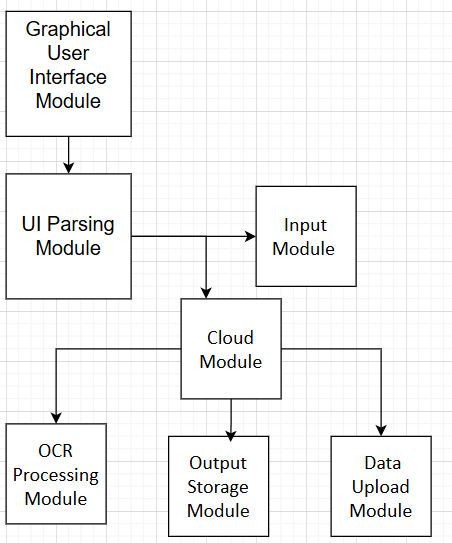
\includegraphics[width=0.7\textwidth]{image.png}
\caption{Use hierarchy among modules}
\label{FigUH}
\end{figure}

%\section*{References}

\section{User Interfaces}
\label{SecUI}

This section presents the graphical user interfaces (GUIs) designed for GradSight. The system is built for a touchscreen display, enabling users to upload, search, and view composite images interactively. The interfaces are powered primarily by Modules M6 (UI Parsing) and M7 (GUI), with support from backend modules for data retrieval and processing.

\begin{figure}[H]
\centering
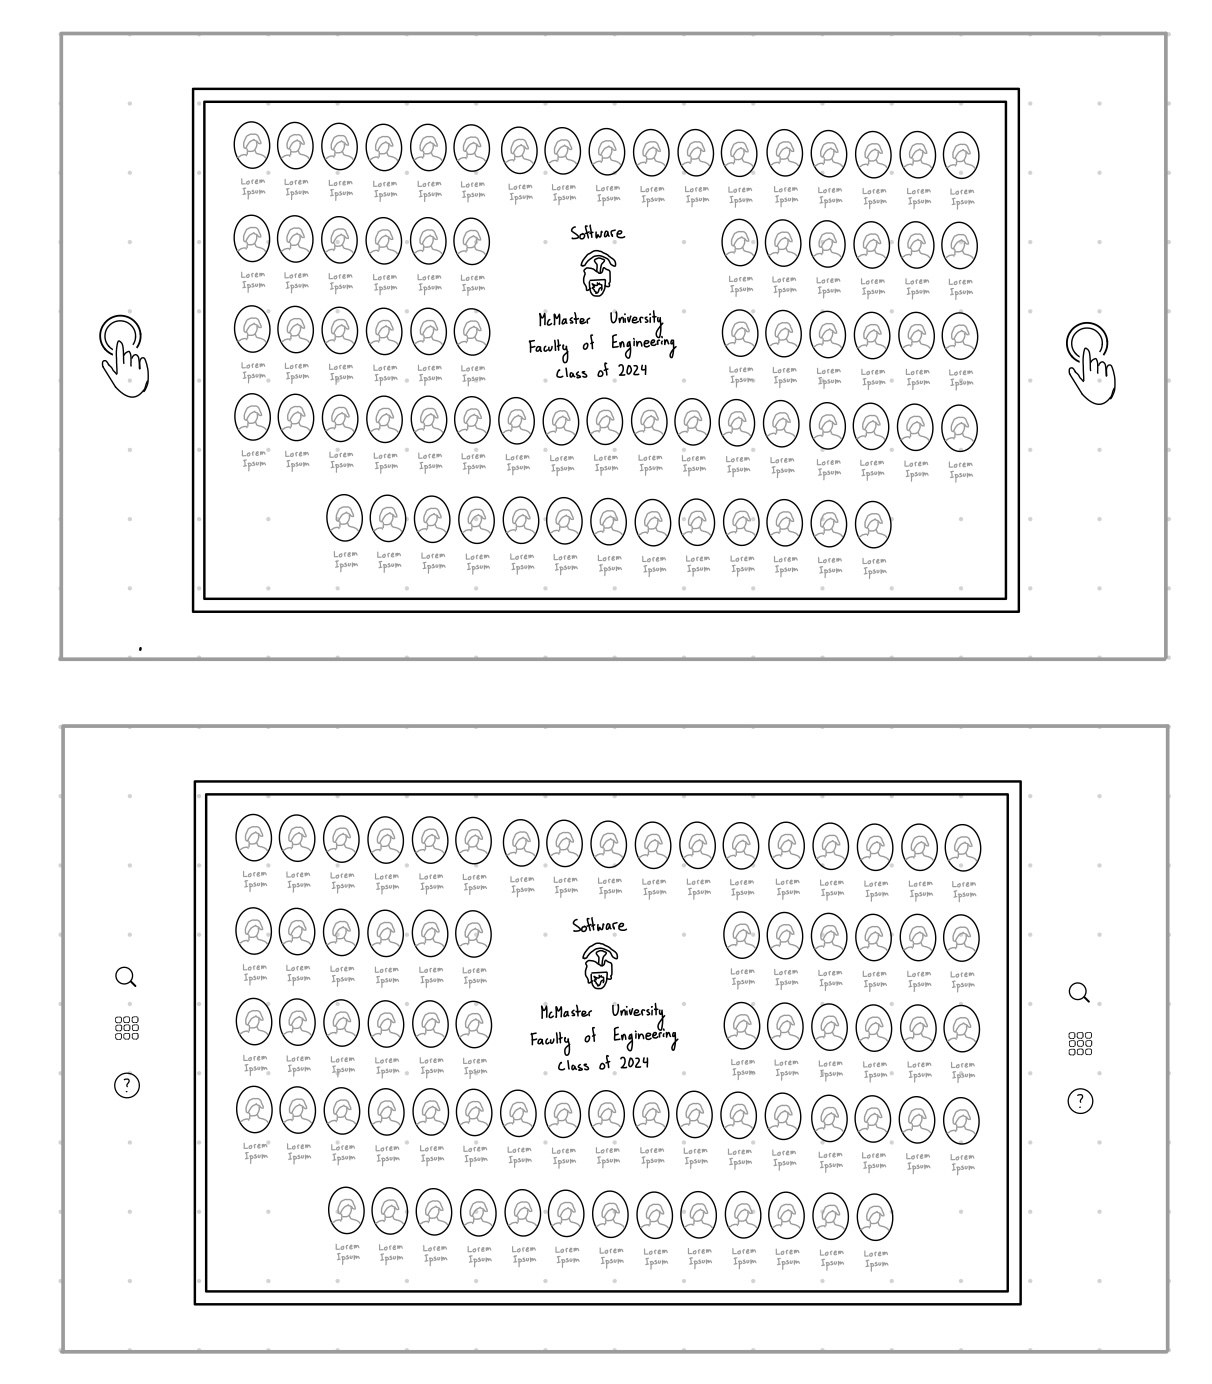
\includegraphics[width=0.7\textwidth]{IMG_0067.png}
\caption{Home Page Interface — The user is presented with an initial menu to choose between Admin and User modes. This screen is managed by M7 (GUI) and determines system flow depending on user role.}
\label{FigUIHome}
\end{figure}

\begin{figure}[H]
\centering
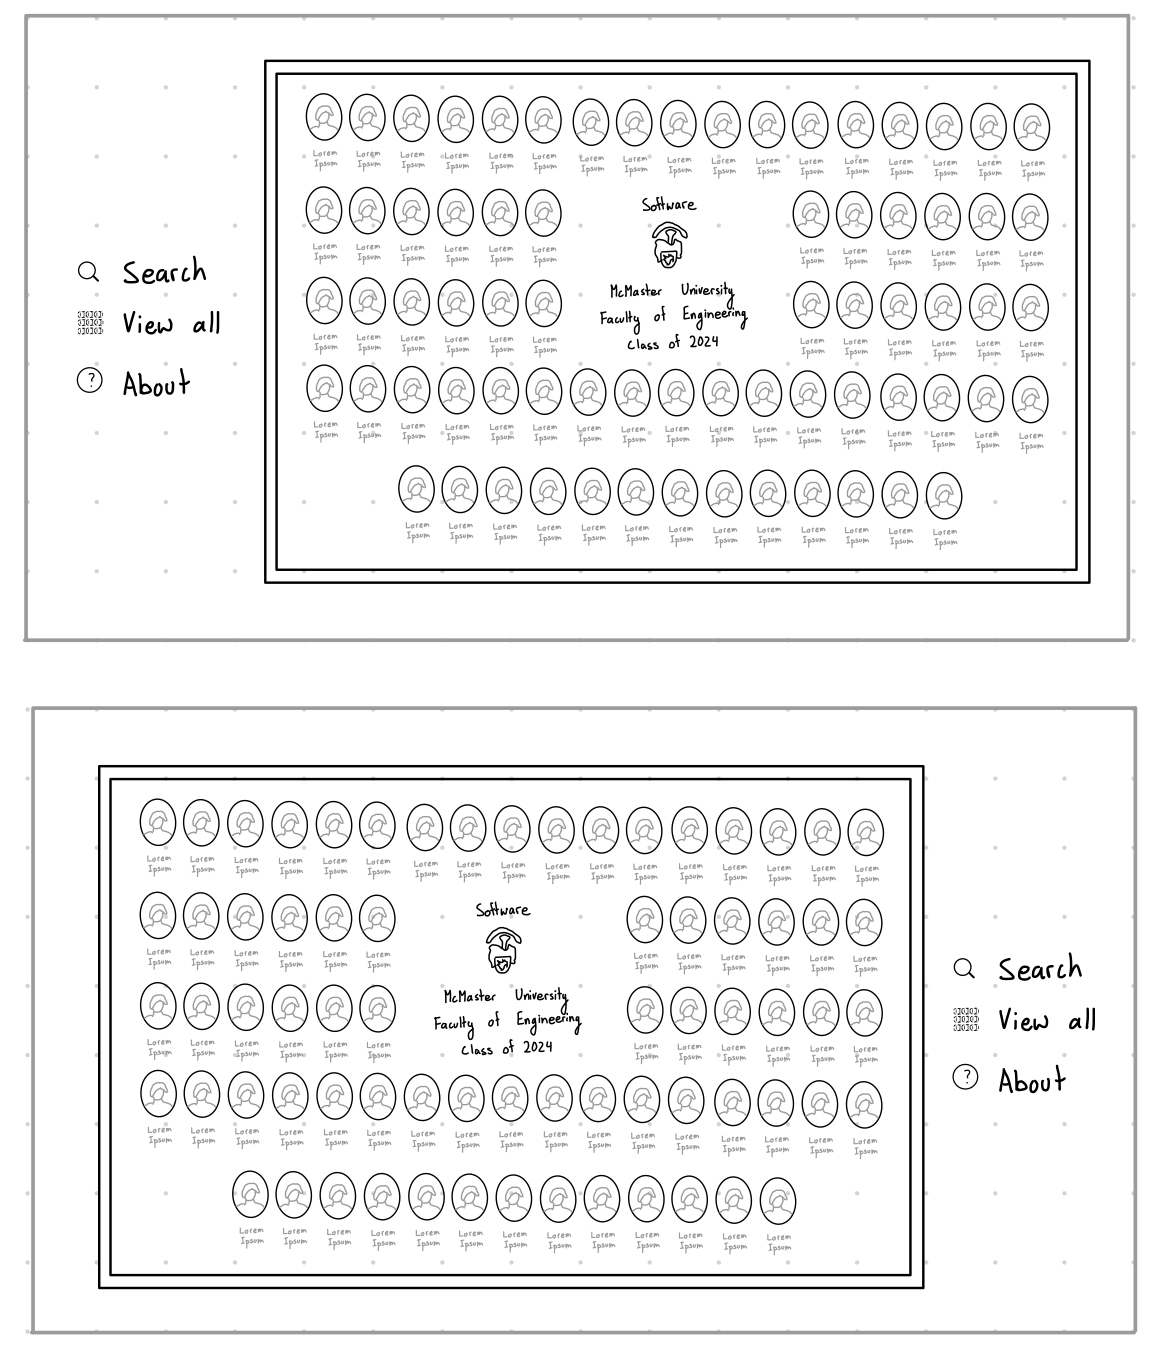
\includegraphics[width=0.7\textwidth]{IMG_0069.png}
\caption{Admin Upload Interface — Admins can upload composite images through this interface. M6 handles file parsing, while M2 and M3 handle input validation and upload logic.}
\label{FigUIUpload}
\end{figure}

\begin{figure}[H]
\centering
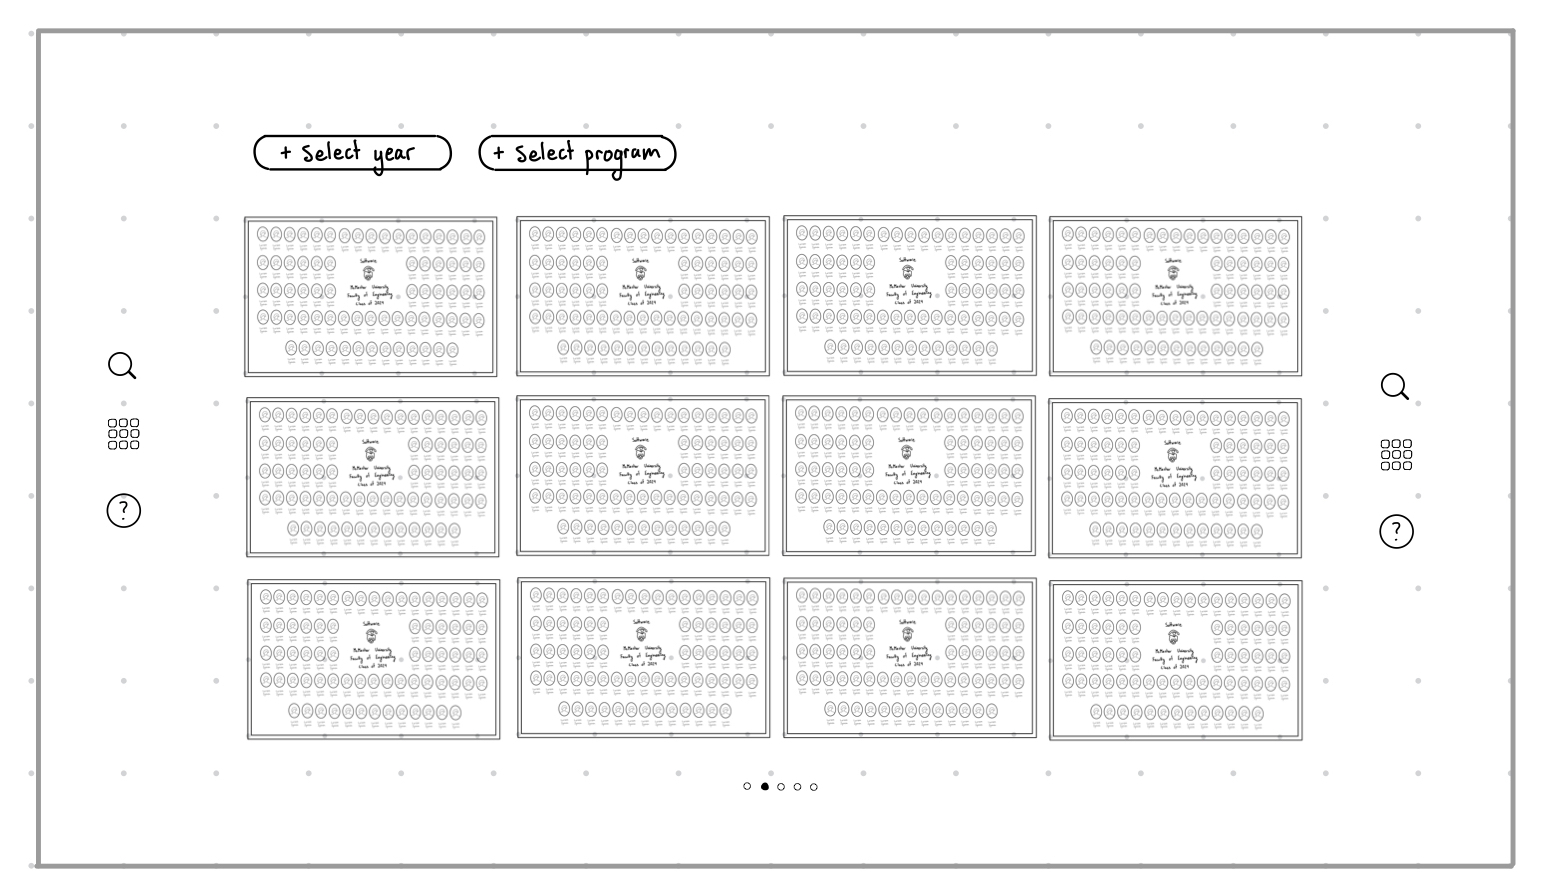
\includegraphics[width=0.7\textwidth]{IMG_0070.png}
\caption{Composite Search Interface — Users can search for individuals by name, program, or year. M7 handles the interactive UI and form input, while M5 retrieves matching data.}
\label{FigUISearch}
\end{figure}

\begin{figure}[H]
\centering
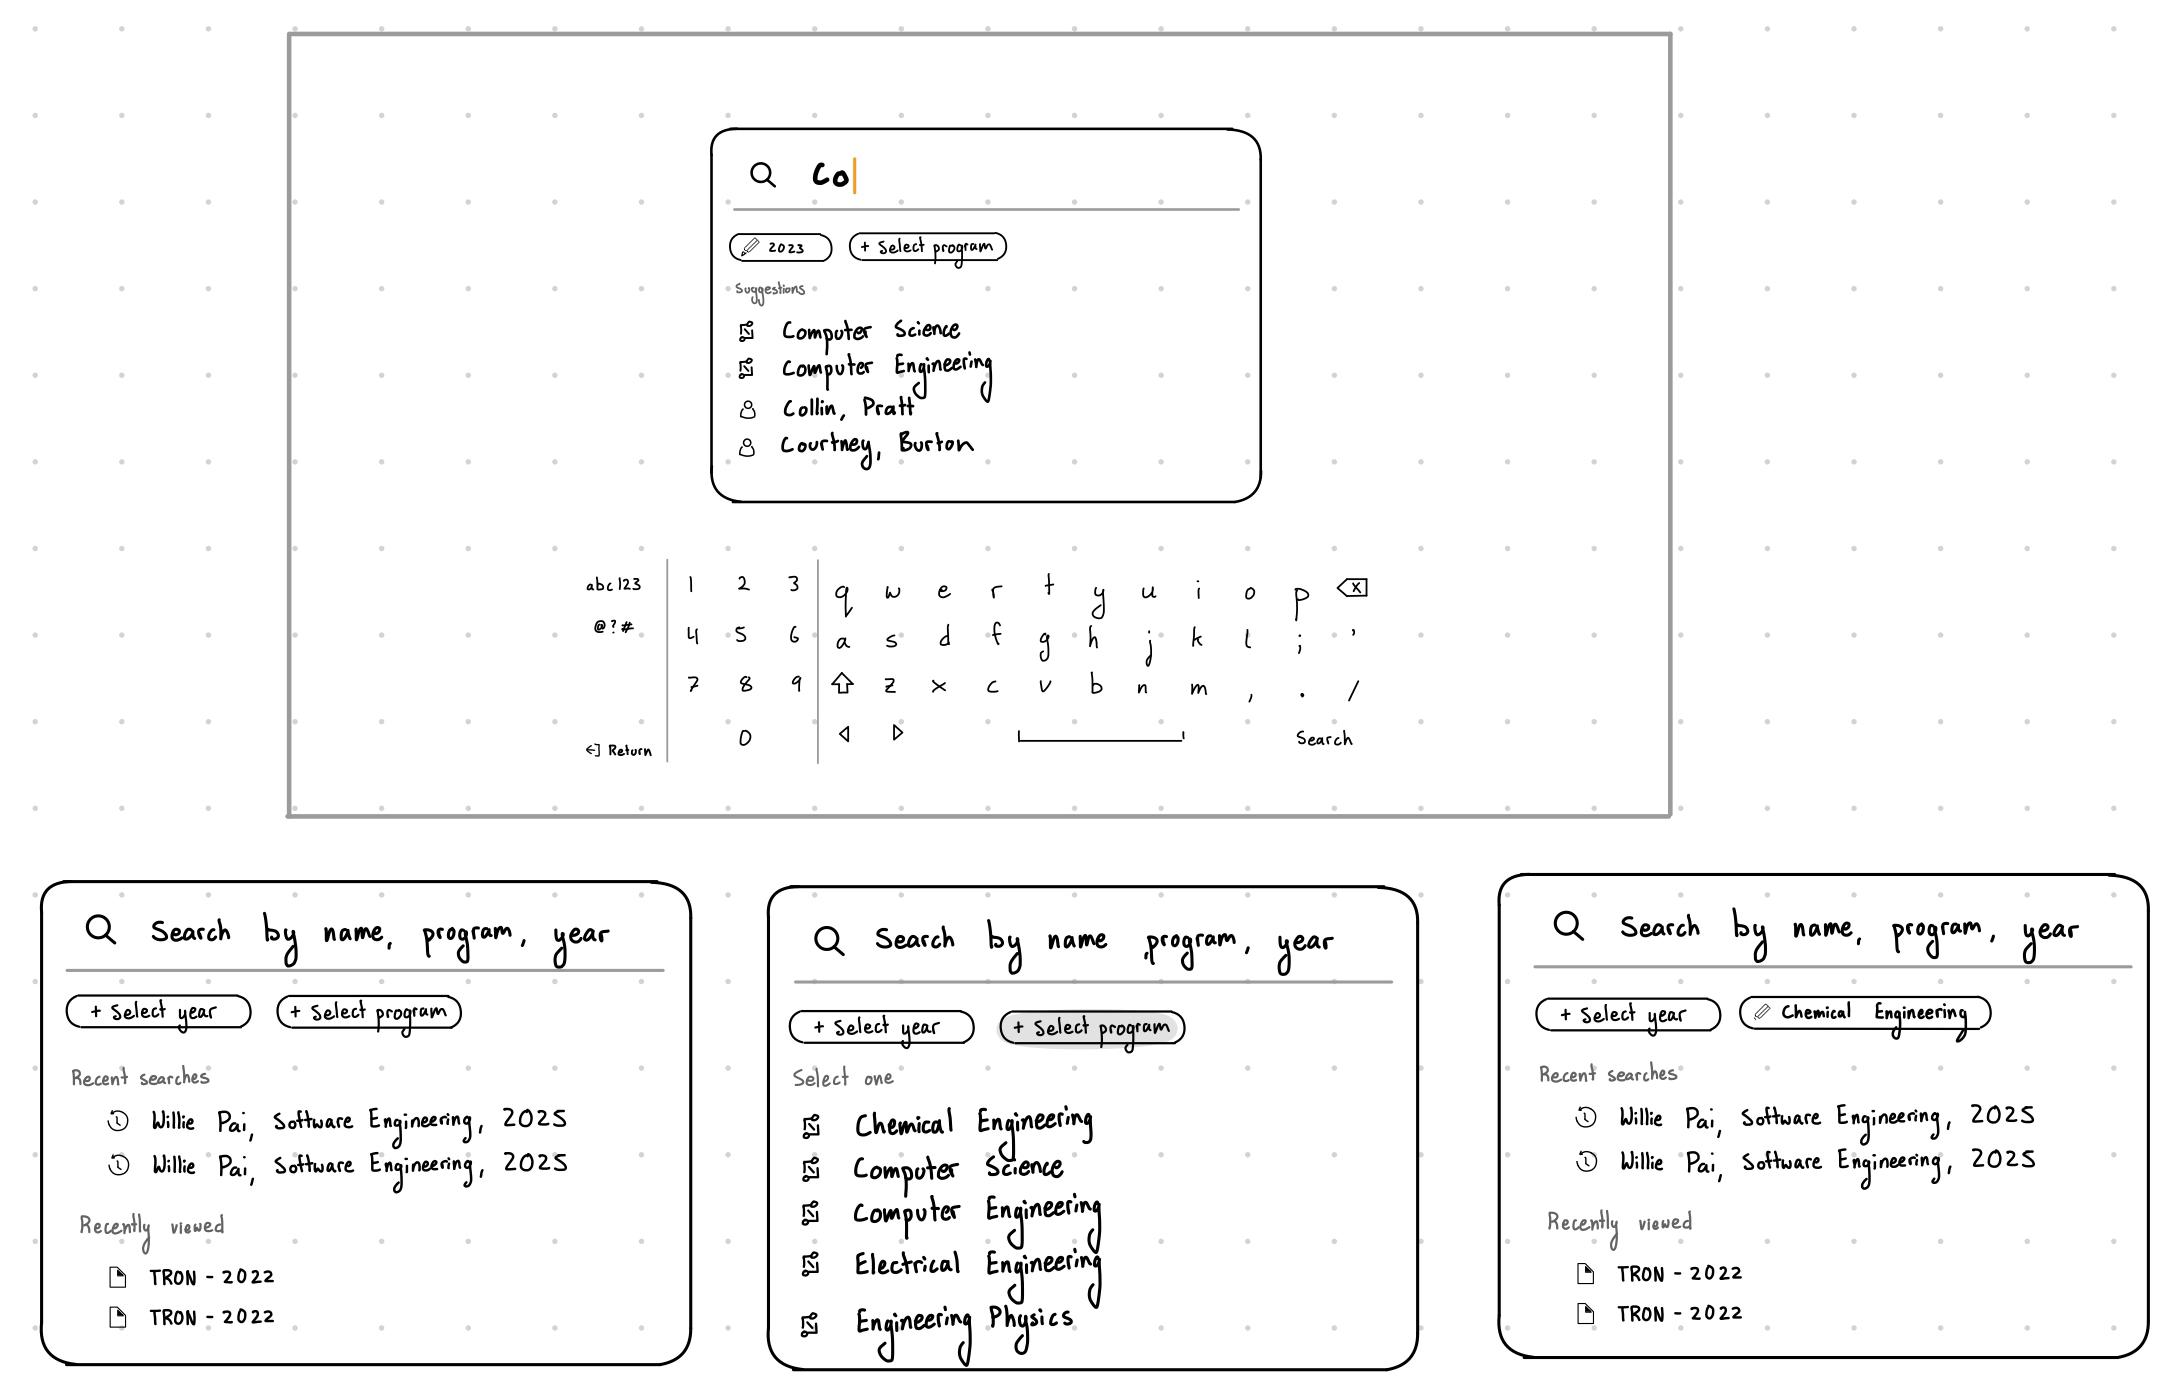
\includegraphics[width=0.7\textwidth]{IMG_0071.png}
\caption{Composite Viewer Interface — The selected composite is displayed with highlights for identified names. This view is rendered by M7 and populated by data from M4 (OCR) and M5 (Output).}
\label{FigUIView}
\end{figure}

\begin{figure}[H]
\centering
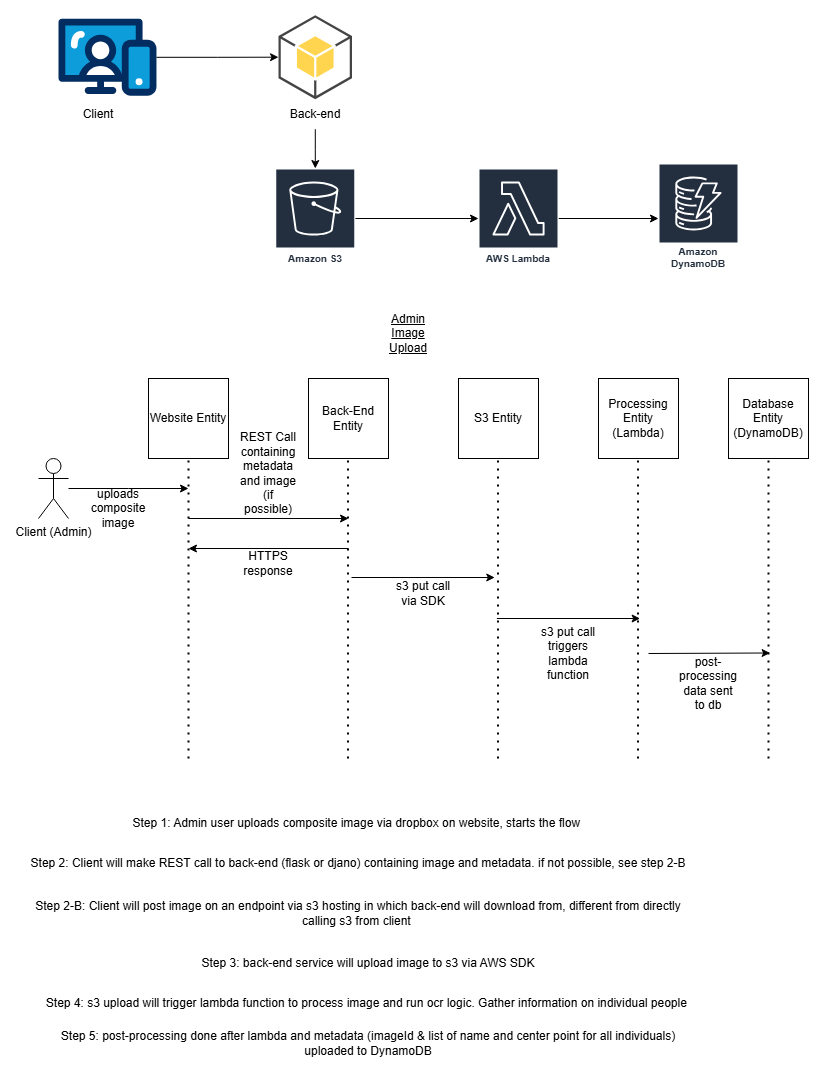
\includegraphics[width=0.7\textwidth]{ocr-arch_1.png}
\caption{Interface Software Architecture — This diagram outlines how the UI interacts with backend services. M6 connects with M2–M5, and M7 manages the front-facing display and user flow.}
\label{FigUIArch}
\end{figure}


\section{Timeline}
\label{SecTimeline}

The development of the GradSight system follows a structured, phase-based schedule designed to ensure a reliable Rev 0 implementation by March. Each phase includes specific deliverables, personnel assignments, and dates. The design emphasizes modular parallelism so team members can develop and test individual components without bottlenecks. Testing is embedded in each phase where appropriate to support early validation.

\subsection{Requirements Gathering and System Design}
\label{SecReq}

\begin{itemize}
  \item \textbf{Sept 23 – Oct 9:} Finalization of software requirements (SRS), hazard analysis, and preliminary architecture planning.
  \item \textbf{Tasks:}
  \begin{itemize}
    \item Define FRs, NFRs, and design constraints.
    \item Complete FMEA and anticipated change table.
    \item Identify modules and interfaces.
  \end{itemize}
  \item \textbf{Leads:} Wajdan (System), Zahin (Hazards), Willie (Comms)
\end{itemize}

\subsection{Front-End and Back-End Development}
\label{SecDev}

Each developer is assigned one or more modules to implement in parallel. Cloud services, OCR pipelines, and database schema are set up early to unblock downstream modules. User interface work starts once the backend API is ready.

\begin{table}[H]
\centering
\caption{Module-Level Development Timeline and Responsibilities}
\label{tab:moduletimeline}
\begin{tabular}{|l|l|l|p{6cm}|}
\hline
\textbf{Module} & \textbf{Developer(s)} & \textbf{Timeline} & \textbf{Responsibility} \\
\hline
M1: Cloud & Henushan & Oct 9--14 & Set up S3, Lambda functions, and DynamoDB with API integration \\
\hline
M2: Input & Wajdan & Oct 12--16 & Validate file structure and convert raw upload into standardized input format \\
\hline
M3: Upload & Zahin, Henushan & Oct 14--18 & Implement frontend upload logic and S3 upload pipeline with error handling \\
\hline
M4: OCR & Hammad, Wajdan & Oct 18--22 & Integrate OCR engine (e.g., Tesseract or Textract) to extract names/coordinates \\
\hline
M5: Output & Henushan & Oct 22--26 & Design database schema and write DynamoDB interface for storing parsed results \\
\hline
M6: UI Parsing & Willie, Hammad & Oct 26--31 & Implement fallback name collection and integrate OCR and database results \\
\hline
M7: GUI & Willie, Zahin & Nov 1--10 & Develop touchscreen interface to navigate and search composite data \\
\hline
\end{tabular}
\end{table}

\subsection{Proof of Concept and Testing}
\label{SecTest}

\begin{itemize}
  \item \textbf{Nov 22 – Feb 3:} Internal testing of core system features. Each module is tested with mock data and then integrated with upstream/downstream modules.
  \item \textbf{Tasks:}
  \begin{itemize}
    \item Unit testing (M2–M5): Hammad
    \item UI testing (M6–M7): Willie
    \item OCR and cloud validation: Zahin
  \end{itemize}
  \item Integration testing begins once the full data pipeline is connected end-to-end.
\end{itemize}

\subsection{Final Deployment and Demonstration}
\label{SecDeploy}

\begin{itemize}
  \item \textbf{Feb 3 – Mar 20:} Final feature polishing, performance improvements, and deployment to production environment.
  \item \textbf{Mar 21 – Mar 30:} Capstone demo preparation, walkthrough testing, UI/UX feedback, poster creation, and video submission.
\end{itemize}

\subsection{Post-Deployment Support and Documentation}
\label{SecSupport}

\begin{itemize}
  \item \textbf{Mar 30 – Apr 2:} Admin onboarding guide, system support documentation, and user-facing instructions.
  \item \textbf{Primary Author:} Hammad (Support), reviewed by Zahin and Willie
\end{itemize}


\newpage{}

\end{document}